\documentclass[conference]{IEEEtran}

\usepackage{amsmath,amssymb,amsfonts}
\usepackage{graphicx}
\usepackage{textcomp}
\usepackage{xcolor}
\usepackage{booktabs}
\usepackage{multirow}
\usepackage{hyperref}
\usepackage{algorithm}
\usepackage{algpseudocode}
\usepackage{subcaption}
\usepackage{url}

\hypersetup{colorlinks=true, linkcolor=blue, citecolor=blue, urlcolor=blue}

\begin{document}

\title{A Controlled Empirical Study of KV Cache Optimization Strategies for Autoregressive LLM Inference}

\author{
\IEEEauthorblockN{Rishika Mamidibathula}
\IEEEauthorblockA{
Columbia University \\
COMS E6998: High Performance Machine Learning \\
rm4318@columbia.edu}
}

\maketitle

\begin{abstract}
Autoregressive inference in large language models is bottlenecked by the key-value (KV) cache, which grows linearly with sequence length and consumes a substantial portion of GPU memory. Several optimization strategies have been proposed---quantization, low-rank approximation, token eviction, and dynamic selection---but direct comparison is difficult because published results use different models, hardware, and evaluation protocols. We present a controlled benchmark that evaluates four representative KV cache optimization techniques (KIVI quantization, xKV SVD decomposition, SnapKV attention-based eviction, and TopK dynamic selection) against an unmodified FP16 baseline on LLaMA-2-7B. All methods share identical model weights, prompts, decode loops, random seeds, and hardware (NVIDIA A100-80GB), isolating the KV cache policy as the sole variable. Our experiments across 120 inference runs at three sequence lengths (512, 2048, 8192 tokens) reveal that no single method dominates across all dimensions. KIVI achieves the highest compression (5.27$\times$ at 2-bit) but incurs significant throughput degradation (56\% slower) due to per-step requantization overhead. SnapKV provides the best throughput-compression tradeoff (3.04$\times$ compression with 8\% faster decoding) but severely degrades generation quality at aggressive budgets. TopK preserves quality perfectly but provides no memory savings by design. xKV SVD offers modest compression (1.40$\times$) with near-lossless quality but reduces throughput by 90\% due to per-head SVD recomputation costs. These findings highlight the absence of a universally optimal KV cache policy and underscore the importance of workload-specific selection.
\end{abstract}

\begin{IEEEkeywords}
KV cache, large language models, inference optimization, memory compression, autoregressive decoding
\end{IEEEkeywords}

\section{Introduction}

The deployment of large language models (LLMs) for real-time text generation presents a fundamental systems challenge: the key-value cache required for autoregressive decoding grows linearly with the number of generated tokens and the input context length. For a model like LLaMA-2-7B with 32 layers and 32 attention heads, the KV cache at a sequence length of 8192 tokens occupies approximately 4.4~GB in FP16---a significant fraction of the GPU memory that could otherwise serve additional concurrent requests or accommodate longer contexts.

This memory pressure has motivated a growing body of work proposing diverse strategies to reduce KV cache footprint: quantizing cache entries to lower bit-widths~\cite{kivi}, compressing them via low-rank decomposition~\cite{xkv}, evicting less important tokens based on attention patterns~\cite{snapkv}, and dynamically selecting subsets of tokens at each decoding step~\cite{topk}. While each approach reports favorable results in isolation, comparing them is challenging because published evaluations differ in model architecture, hardware platform, batch size, sequence length distribution, and quality metrics.

This work addresses the comparability gap through a controlled benchmark with the following design principles:

\begin{itemize}
    \item \textbf{Single variable}: All methods share the same model weights, tokenizer, prompt set, decode loop, random seeds, and GPU hardware. The only variable across experiments is the KV cache policy.
    \item \textbf{Unified measurement}: Every run reports the same six metrics---peak GPU memory, KV cache size, compression ratio, time-to-first-token (TTFT), per-token decode latency, and throughput---using identical instrumentation.
    \item \textbf{Fair quality evaluation}: Perplexity is measured using a split-text protocol where all methods (including the baseline) prefill the first half of a passage, apply their KV modification, and are evaluated on the second half. This ensures the same evaluation conditions for every technique.
    \item \textbf{Pure algorithmic overhead}: All implementations use standard PyTorch operations without custom CUDA or Triton kernels, isolating the algorithmic cost of each approach from kernel-level optimizations that vary across implementations.
\end{itemize}

Our benchmark encompasses 120 synthetic inference runs across 12 hyperparameter configurations and 12 perplexity evaluations on WikiText-103, executed on Modal cloud compute with NVIDIA A100-80GB GPUs. The results reveal a multi-dimensional tradeoff space where each method occupies a distinct region, and the optimal choice depends on whether the deployment prioritizes memory efficiency, throughput, or output quality.

\section{Related Work}

\subsection{KV Cache Quantization}
KIVI~\cite{kivi} introduced asymmetric quantization for KV caches, observing that key tensors exhibit outliers along the channel dimension while value tensors have outliers along the token dimension. This motivates per-channel quantization for keys and per-token quantization for values, with a sliding window of recent tokens retained in full precision. The original implementation uses custom Triton kernels for fused quantized attention; our benchmark evaluates the algorithmic approach using standard PyTorch operations.

\subsection{Low-Rank Approximation}
xKV~\cite{xkv} exploits the observation that KV cache tensors across layers share a common low-dimensional subspace. The method applies truncated SVD to compress KV representations, storing the decomposed components (U, S, V$^{\top}$) instead of full matrices. The original paper proposes cross-layer grouping to amortize SVD cost; our implementation applies per-layer, per-head SVD for simplicity and evaluates the compression-quality tradeoff at different rank settings.

\subsection{Attention-Based Eviction}
SnapKV~\cite{snapkv} performs a one-time eviction step after the prefill phase. It analyzes the attention weight distribution from the prefill computation to identify which tokens received the most cumulative attention, retaining a fixed budget of important tokens along with ``attention sink'' positions (typically the first few tokens) and a window of recent tokens. Evicted tokens are permanently discarded, reducing both memory and computation for all subsequent decode steps.

\subsection{Dynamic Token Selection}
TokenSelect~\cite{topk} takes a different approach by maintaining the full KV cache but restricting attention computation to a dynamically chosen subset at each decode step. Using the query vector from the current step, it scores all cached positions via a lightweight dot-product approximation and selects the top-K most relevant tokens for the full attention computation. This preserves the ability to attend to any historical token while reducing per-step compute.

\subsection{Other Approaches}
Several other methods have been proposed, including H2O~\cite{h2o} which uses cumulative attention scores to identify ``heavy hitter'' tokens for retention, PyramidKV~\cite{pyramidkv} which allocates different cache budgets across layers, and StreamingLLM~\cite{streamingllm} which maintains a fixed-size sliding window with attention sinks. While we do not evaluate all of these, our benchmark framework is extensible and can accommodate additional methods through its modular wrapper interface.

\section{Methodology}

\subsection{Benchmark Architecture}

We implement a unified benchmark framework where each KV cache optimization technique conforms to a common abstract interface (\texttt{MethodWrapper}) exposing four operations:

\begin{itemize}
    \item \texttt{process\_prefill(past\_kv, attn\_weights)}: Modify the KV cache immediately after the prefill forward pass.
    \item \texttt{process\_step(past\_kv, step, attn\_weights)}: Modify the KV cache after each autoregressive decode step.
    \item \texttt{get\_kv\_size\_bytes(past\_kv)}: Report the actual memory footprint of the method's internal cache representation.
    \item \texttt{reset()}: Clear internal state between runs.
\end{itemize}

This abstraction ensures that the generation loop---including tokenization, forward passes, next-token selection, and timing instrumentation---is identical across all methods. The only variation is the cache transformation applied at each step.

\subsection{DynamicCache Compatibility}

A practical challenge arises from HuggingFace Transformers (v4.36+) transitioning from plain tuple representations of \texttt{past\_key\_values} to \texttt{DynamicCache} objects. Our methods operate on tuple format (lists of per-layer key-value tensor pairs), so we implement bidirectional conversion utilities: \texttt{DynamicCache} $\rightarrow$ tuple before invoking method hooks, and tuple $\rightarrow$ \texttt{DynamicCache} before returning modified caches to the model. This allows our benchmark to work with current Transformers versions without requiring methods to handle framework-specific cache classes.

\subsection{Method Implementations}

\subsubsection{KIVI Quantization}
Our KIVI implementation performs asymmetric quantization at configurable bit-widths (2-bit and 4-bit). Keys are quantized per-channel (along the head dimension) and values per-token (along the sequence dimension), following the asymmetry identified in~\cite{kivi}. A sliding window of \texttt{residual\_length}=128 most recent tokens is maintained in FP16. At each decode step, the oldest token in the residual window overflows into the quantized buffer, which is re-quantized to absorb the new entry. The reported KV cache size accounts for the true bit-width: $\text{size} = \text{numel} \times \text{bits} / 8$ bytes for quantized tensors, plus scale, zero-point, and residual overhead in FP16.

\subsubsection{xKV SVD Decomposition}
We implement per-head truncated SVD on KV tensors. For each attention head, the key matrix $K_h \in \mathbb{R}^{T \times d}$ is decomposed as $K_h \approx U_r \Sigma_r V_r^{\top}$ where $r$ is the target rank. We store $U_r \in \mathbb{R}^{T \times r}$, $\Sigma_r \in \mathbb{R}^r$, and $V_r \in \mathbb{R}^{r \times d}$ in FP16. Values receive a higher rank budget ($r_v = 1.5 \times r_k$) since they are empirically less compressible. New tokens accumulate in a residual buffer; every \texttt{recompute\_interval}=50 steps, the full cache is reconstructed, combined with the residual, and re-decomposed.

\subsubsection{SnapKV Eviction}
SnapKV performs a single eviction pass after prefill using the attention weight matrices from the prefill forward pass. For each layer and head, it computes an importance score per token position by averaging attention weights within an observation window of the last 32 positions. It retains: (1) the first \texttt{sink\_size}=4 tokens (attention sinks), (2) the top-scoring tokens up to the budget, and (3) a window of recent tokens. This requires setting \texttt{output\_attentions=True} during prefill, which materializes the full $T \times T$ attention matrix and limits scalability to shorter sequences (OOM at 8192 tokens on A100-80GB).

\subsubsection{TopK Dynamic Selection}
At each decode step, TopK scores all cached positions using the proxy dot-product $q \cdot K^{\top}$ computed from the last layer's key cache. The top-K highest-scoring positions are selected, combined with the 16 most recent positions (recency bias), and returned as the active cache for attention computation. Crucially, the full cache is always maintained internally---TopK trades per-step computation for quality preservation, not memory for quality. Every \texttt{refresh\_interval} steps, the full cache is passed to attention for a complete context refresh.

\subsection{Perplexity Evaluation Protocol}

To measure quality degradation from KV cache modifications, we employ a split-text protocol uniformly across all methods, including the baseline:

\begin{enumerate}
    \item Tokenize a WikiText-103 passage (up to 512 tokens).
    \item Split into two halves: context tokens $x_{1:T/2}$ and evaluation tokens $x_{T/2+1:T}$.
    \item Run a prefill forward pass on the context tokens to populate the KV cache.
    \item Apply the method's \texttt{process\_prefill} hook to modify the cache.
    \item Run a forward pass on the evaluation tokens using the modified cache with teacher-forced labels.
    \item Compute cross-entropy loss on the evaluation tokens.
\end{enumerate}

Using the same protocol for all methods, including baseline, ensures that perplexity values are directly comparable. A method that perfectly preserves cache fidelity will match baseline perplexity; degradation indicates information loss from the optimization.

\subsection{Experimental Setup}

\begin{itemize}
    \item \textbf{Model}: Meta LLaMA-2-7B (\texttt{meta-llama/Llama-2-7b-hf}), FP16 inference, 32 layers, 32 heads, head dimension 128.
    \item \textbf{Hardware}: NVIDIA A100-80GB (Modal cloud compute), one GPU per method configuration.
    \item \textbf{Prompts}: 12 synthetic prompts constructed from WikiText-103 training data, 4 per target sequence length (512, 2048, 8192 tokens), each wrapped with a summarization instruction prefix.
    \item \textbf{Decoding}: Greedy (argmax), \texttt{max\_new\_tokens}=200, batch size 1.
    \item \textbf{Seeds}: \texttt{torch.manual\_seed(42)} before every run.
    \item \textbf{Timing}: \texttt{torch.cuda.synchronize()} around all measurements, wall-clock via \texttt{time.perf\_counter()}.
    \item \textbf{Memory}: \texttt{torch.cuda.reset\_peak\_memory\_stats()} before each run.
    \item \textbf{Parallelism}: All method configurations execute simultaneously on separate GPU containers via Modal's serverless infrastructure, with baseline running serially first to establish KV cache size denominators.
\end{itemize}

\section{Results}

We report results from 120 synthetic inference runs (10 method-config combinations $\times$ 12 prompts, minus SnapKV and xKV failures at 8192 tokens) and 12 perplexity evaluations on WikiText-103.

\subsection{Compression and Memory}

Table~\ref{tab:main_results} presents the aggregate results across all sequence lengths. KIVI at 2-bit achieves the highest compression ratio of 5.27$\times$, reducing the average KV cache from 1990.7~MB to 323.1~MB. At 4-bit, KIVI still provides substantial compression (3.20$\times$). SnapKV at budget=0.2 achieves 3.04$\times$ compression through aggressive token eviction. xKV with rank=64 provides modest compression at 1.40$\times$, while rank=128 and rank=256 offer no effective compression (0.90$\times$) because the SVD component storage overhead exceeds the savings when the rank approaches the head dimension (128).

\begin{table}[t]
\centering
\caption{Aggregate benchmark results across all sequence lengths. Compression ratio is relative to baseline FP16 KV cache size. PPL measured via split-text protocol on WikiText-103.}
\label{tab:main_results}
\begin{tabular}{@{}llrrrrr@{}}
\toprule
\textbf{Method} & \textbf{Config} & \textbf{KV} & \textbf{Comp.} & \textbf{TPS} & \textbf{Lat.} & \textbf{PPL} \\
 & & \textbf{(MB)} & \textbf{ratio} & & \textbf{(ms)} & \\
\midrule
Baseline & FP16 & 1990.7 & 1.00$\times$ & 32.9 & 30.5 & 6.94 \\
\midrule
KIVI & 4-bit, res=128 & 563.6 & 3.20$\times$ & 16.7 & 93.7 & 6.93 \\
KIVI & 2-bit, res=128 & 323.1 & 5.27$\times$ & 14.6 & 98.8 & 13.70 \\
\midrule
xKV & rank=64 & 541.1 & 1.40$\times$ & 3.3 & 305.6 & 7.12 \\
xKV & rank=128 & 850.4 & 0.90$\times$ & 3.0 & 333.7 & 6.94 \\
\midrule
SnapKV & budget=0.6 & 511.4 & 1.49$\times$ & 38.3 & 26.2 & 12.78 \\
SnapKV & budget=0.4 & 375.9 & 1.99$\times$ & 50.1 & 20.0 & 27.16 \\
SnapKV & budget=0.2 & 240.4 & 3.04$\times$ & 35.6 & 28.4 & 29.41 \\
\midrule
TopK & K=256 & 1990.7 & 1.00$\times$ & 35.7 & 29.5 & 6.94 \\
TopK & K=512 & 1990.7 & 1.00$\times$ & 26.4 & 39.0 & 6.94 \\
TopK & K=1024 & 1990.7 & 1.00$\times$ & 29.0 & 36.4 & 6.94 \\
\bottomrule
\end{tabular}
\end{table}

TopK shows a compression ratio of exactly 1.00$\times$ across all configurations, confirming its design principle of maintaining the complete cache for quality preservation while only varying the attention computation.

\subsection{Compression Scaling with Sequence Length}

Table~\ref{tab:seq_scaling} shows how compression ratios evolve with input sequence length. KIVI compression improves significantly at longer sequences because the fixed-size FP16 residual window (128 tokens) becomes a smaller fraction of the total cache. At 8192 tokens, KIVI 2-bit achieves 6.84$\times$ compression compared to 3.48$\times$ at 512 tokens. SnapKV compression similarly improves with length since the fixed retention budget represents a smaller fraction of longer sequences.

\begin{table}[t]
\centering
\caption{Compression ratio by sequence length for each method's best configuration.}
\label{tab:seq_scaling}
\begin{tabular}{@{}lrrr@{}}
\toprule
\textbf{Method} & \textbf{512} & \textbf{2048} & \textbf{8192} \\
\midrule
Baseline & 1.00$\times$ & 1.00$\times$ & 1.00$\times$ \\
KIVI 2-bit & 3.48$\times$ & 5.48$\times$ & 6.84$\times$ \\
KIVI 4-bit & 2.56$\times$ & 3.33$\times$ & 3.71$\times$ \\
SnapKV 0.2 & 2.38$\times$ & 3.69$\times$ & --- \\
xKV rank=64 & 1.31$\times$ & 1.50$\times$ & --- \\
TopK K=256 & 1.00$\times$ & 1.00$\times$ & 1.00$\times$ \\
\bottomrule
\end{tabular}
\end{table}

SnapKV and xKV entries at 8192 tokens are absent because both methods encountered errors at this sequence length---SnapKV due to OOM when materializing full attention weight matrices ($32 \times 32 \times 8192 \times 8192$ in FP16 $\approx$ 137~GB), and xKV due to numerical instability in per-head SVD at large matrix sizes.

\subsection{Throughput and Latency}

The throughput results reveal a clear hierarchy. SnapKV at budget=0.4 achieves the highest throughput (50.1 tokens/sec), exceeding baseline (32.9 tokens/sec) by 52\%. This acceleration occurs because eviction reduces the KV cache size, which in turn reduces the attention computation at every subsequent decode step. TopK at K=256 achieves 35.7 tokens/sec, slightly above baseline, because the reduced attention set offsets the scoring overhead.

KIVI incurs substantial throughput degradation (16.7 TPS at 4-bit, 14.6 TPS at 2-bit), representing a 49--56\% slowdown. This overhead stems from the per-step dequantize--attend--requantize cycle implemented in pure PyTorch. The original KIVI paper~\cite{kivi} reports throughput gains through custom Triton kernels that fuse quantized attention; our results isolate the algorithmic overhead without such kernel optimizations.

xKV exhibits the most severe throughput impact at 3.0--3.5 TPS (90\% slower than baseline). The bottleneck is the per-head SVD decomposition: at each recomputation step, \texttt{torch.linalg.svd} is invoked 32 times per layer $\times$ 32 layers = 1024 times for keys alone, with an equivalent cost for values. The TTFT for xKV reaches 10--12 seconds at 512 tokens due to the initial prefill SVD, compared to 0.05--0.4 seconds for other methods.

\subsection{Quality Degradation}

Perplexity results on WikiText-103 (Table~\ref{tab:main_results}) show three distinct quality tiers:

\textbf{Lossless} (PPL $\approx$ baseline 6.94): KIVI 4-bit (6.93), xKV rank$\geq$128 (6.94), and all TopK configurations (6.94) preserve generation quality. For KIVI 4-bit, the quantization error at 4 bits per value is below the model's inherent noise floor. For xKV at rank=128, the SVD retains all 128 singular values (equal to head\_dim), so no information is lost. TopK always attends to the full cache at refresh steps and selects the most query-relevant tokens otherwise, preserving the model's attention distribution.

\textbf{Mild degradation} (PPL 7--13): KIVI 2-bit (13.70) and xKV rank=64 (7.12) show measurable but bounded quality loss. The 2-bit quantization introduces significant rounding error, approximately doubling perplexity relative to baseline. xKV rank=64 discards roughly half the singular spectrum per head, losing fine-grained contextual information while retaining the dominant patterns.

\textbf{Severe degradation} (PPL $>$ 12): SnapKV at all tested budgets shows substantial quality loss (12.78--29.41). Even at the most generous budget (0.6, retaining 60\% of tokens), perplexity nearly doubles. This suggests that the attention-pattern-based importance scoring, while effective for identifying globally important tokens, systematically discards tokens that carry information needed for coherent generation in the evaluation window. The one-shot nature of SnapKV's eviction (no opportunity to recover discarded tokens) makes it particularly sensitive to scoring errors.

\subsection{Peak GPU Memory}

An unexpected finding is that KIVI's peak GPU memory (26.1~GB average) exceeds baseline (20.5~GB) despite achieving the highest KV cache compression. This apparent contradiction arises because KIVI's per-step dequantize--requantize cycle creates temporary FP16 tensors (the dequantized historical cache concatenated with the residual window) that exist simultaneously with the quantized cache. The peak memory therefore reflects the high-water mark of these transient allocations rather than the steady-state compressed cache size. In a production system with fused kernels that quantize in-place, this overhead would be eliminated.

SnapKV and xKV show peak memory comparable to or lower than baseline at their supported sequence lengths, confirming that cache size reduction translates to memory savings when the method's internal operations do not create large temporaries.

\section{Discussion}

\subsection{The Pareto Frontier}

\begin{figure}[t]
    \centering
    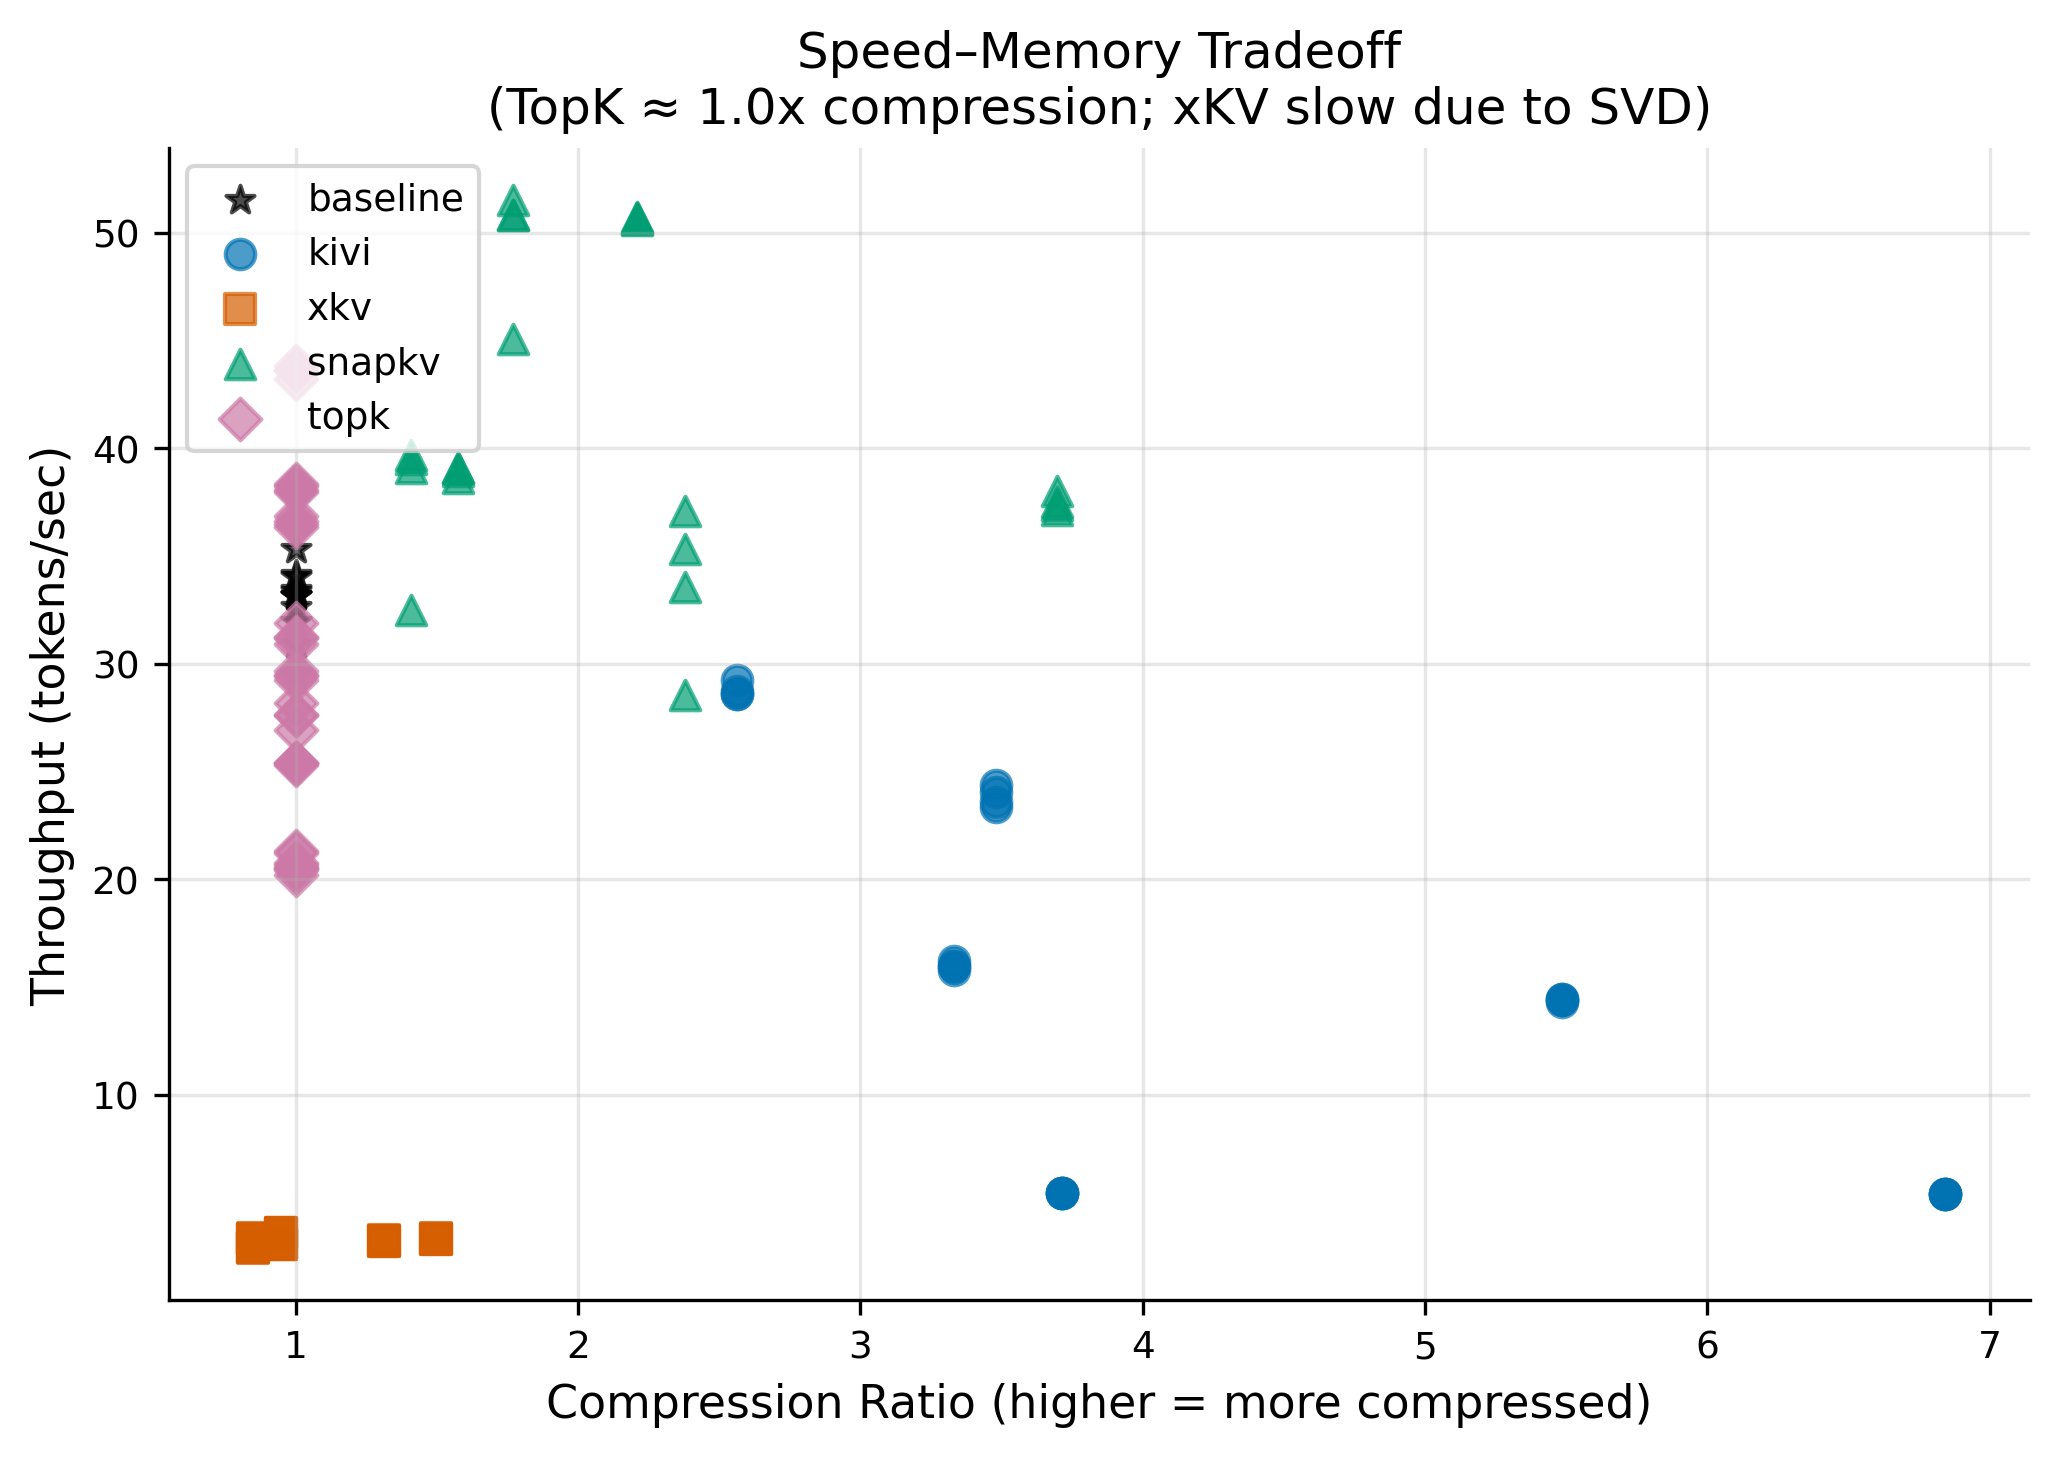
\includegraphics[width=\columnwidth]{../results/plots/throughput_vs_compression.png}
    \caption{Throughput vs. compression ratio. Each point represents one (method, config, seq\_len) combination. The Pareto-optimal region is the upper-right quadrant (high compression, high throughput). SnapKV at moderate budgets occupies this region; KIVI achieves high compression but at reduced throughput; xKV falls in the low-throughput region.}
    \label{fig:throughput_compression}
\end{figure}

No single method dominates across all three dimensions of the memory--throughput--quality tradeoff:

\begin{itemize}
    \item \textbf{Memory-constrained deployments} where serving cost is dominated by KV cache VRAM: KIVI 2-bit offers the best compression (5.27$\times$) with acceptable quality (PPL 13.70) if throughput degradation is tolerable.
    \item \textbf{Throughput-sensitive serving} where tokens-per-second determines user-facing latency: SnapKV at budget=0.4 provides 52\% throughput improvement with 1.99$\times$ compression, though quality monitoring is essential.
    \item \textbf{Quality-critical applications} where output fidelity cannot be compromised: TopK at K=256 provides a modest 8\% throughput improvement over baseline while preserving quality perfectly, at the cost of no memory savings.
\end{itemize}

\subsection{Algorithmic vs.\ Kernel-Level Overhead}

Our deliberate choice to implement all methods in pure PyTorch---without custom CUDA or Triton kernels---has important implications for interpreting the throughput results. KIVI's 49\% throughput reduction and xKV's 90\% reduction reflect the cost of Python-level quantization arithmetic and SVD computation, respectively. Production implementations with fused kernels would substantially reduce these overheads. However, the \textit{relative} ranking of methods by algorithmic complexity (SnapKV $<$ TopK $<$ KIVI $<$ xKV) is likely to be preserved even with kernel-level optimization, since the fundamental operations (eviction/selection vs.\ quantization vs.\ matrix decomposition) differ in computational complexity.

\subsection{Scalability Limitations}

Both SnapKV and xKV failed at our longest sequence length (8192 tokens), though for different reasons. SnapKV's requirement for full attention weight matrices scales as $O(T^2)$ in memory, making it fundamentally incompatible with very long sequences on memory-limited hardware without architectural modifications (e.g., chunked attention scoring). xKV's per-head SVD encounters numerical precision issues with large matrices in FP16. These scalability gaps represent meaningful limitations for production deployment where input lengths are variable and unpredictable.

\begin{figure}[t]
    \centering
    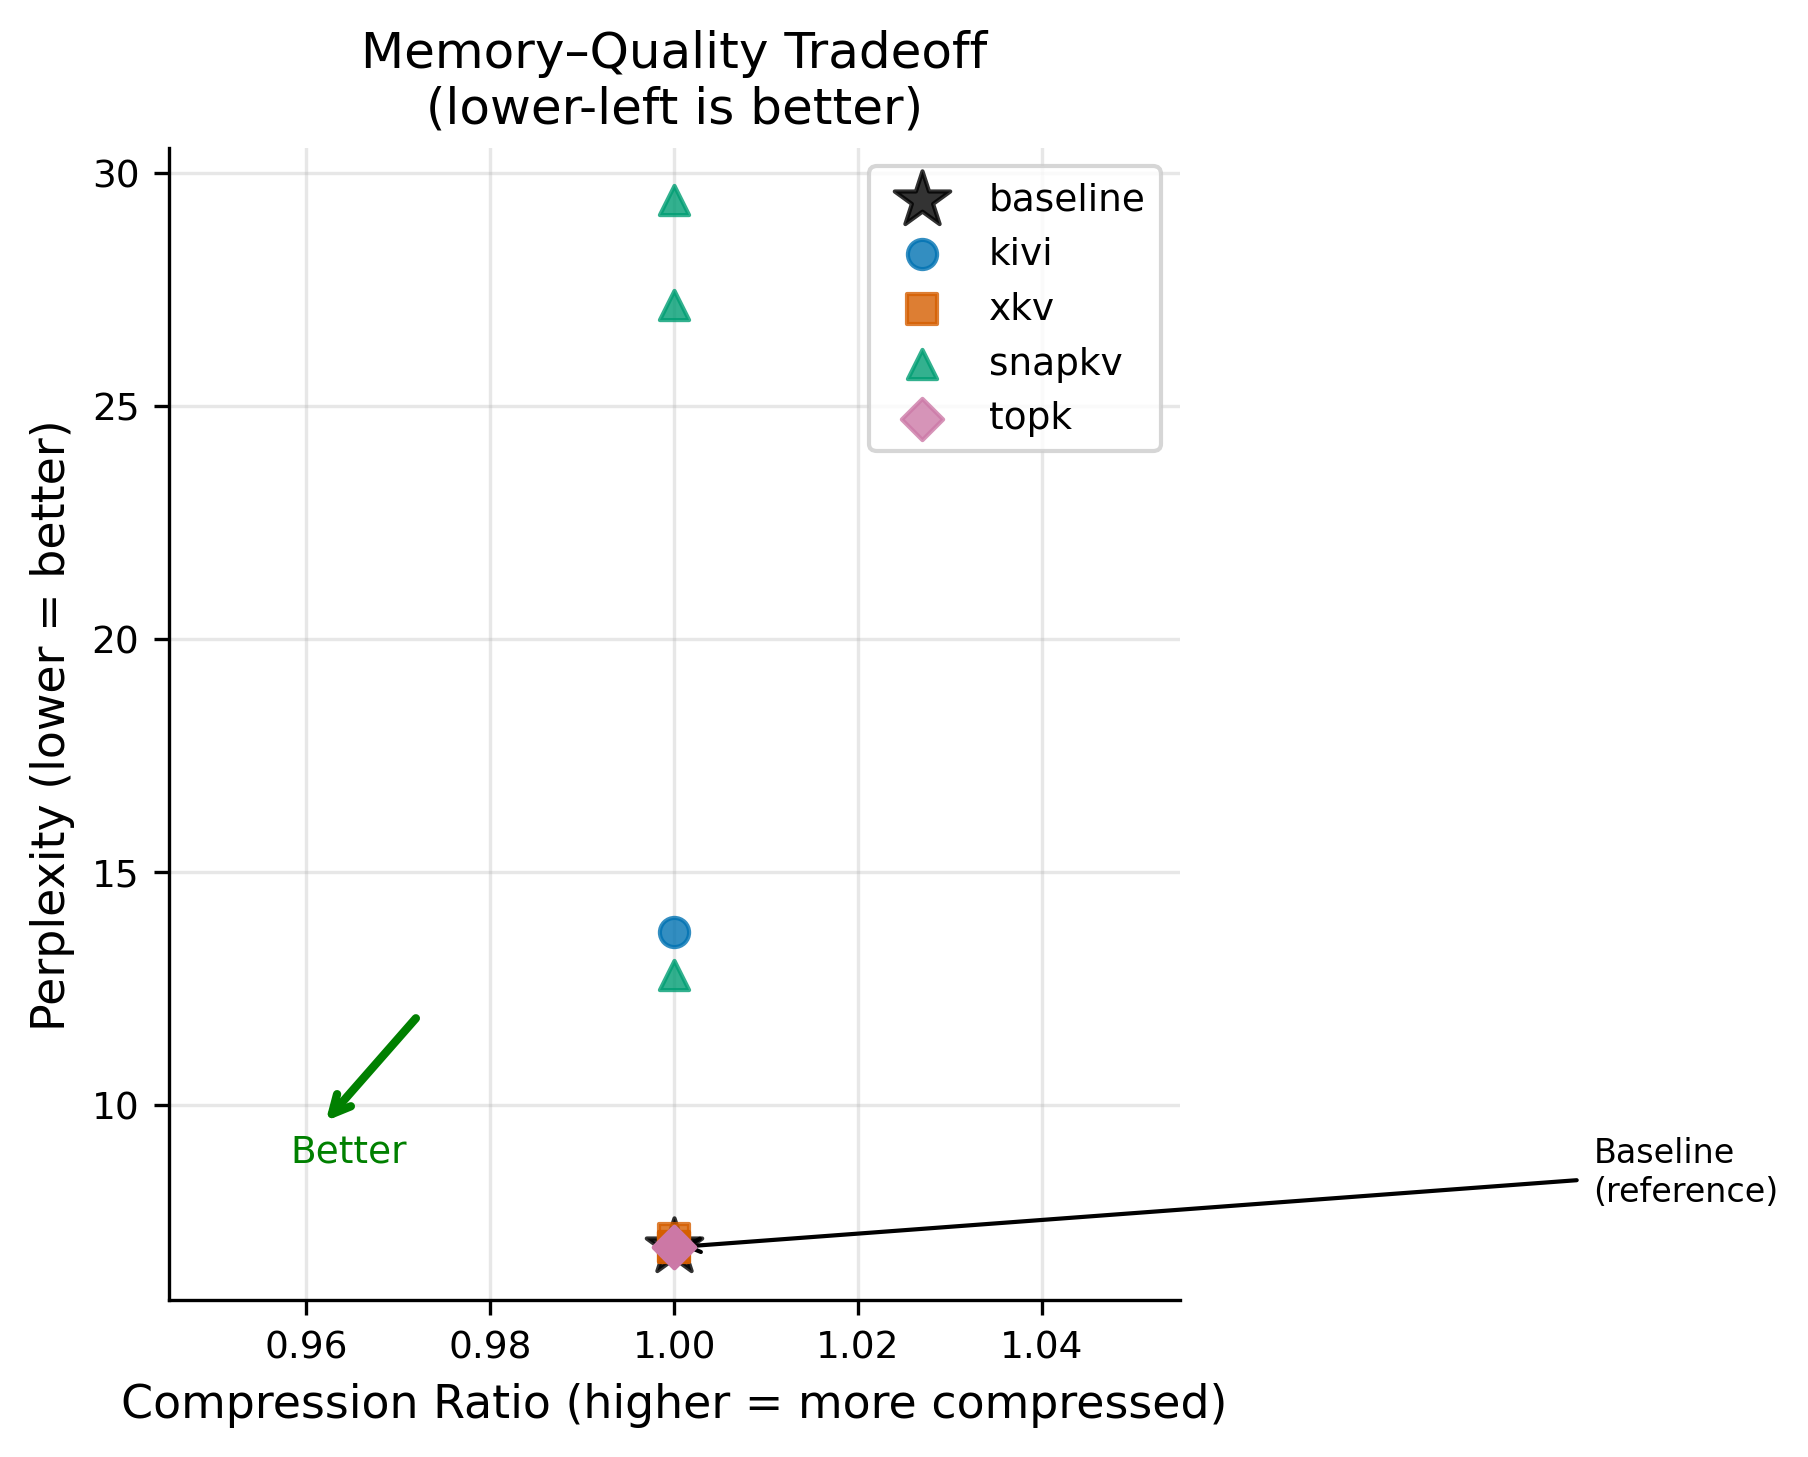
\includegraphics[width=\columnwidth]{../results/plots/memory_vs_quality.png}
    \caption{Memory--quality tradeoff. Compression ratio vs.\ perplexity for each method configuration. The ideal region is the lower-right (high compression, low perplexity). KIVI 4-bit and xKV rank=64 achieve meaningful compression with minimal quality impact.}
    \label{fig:memory_quality}
\end{figure}

\begin{figure}[t]
    \centering
    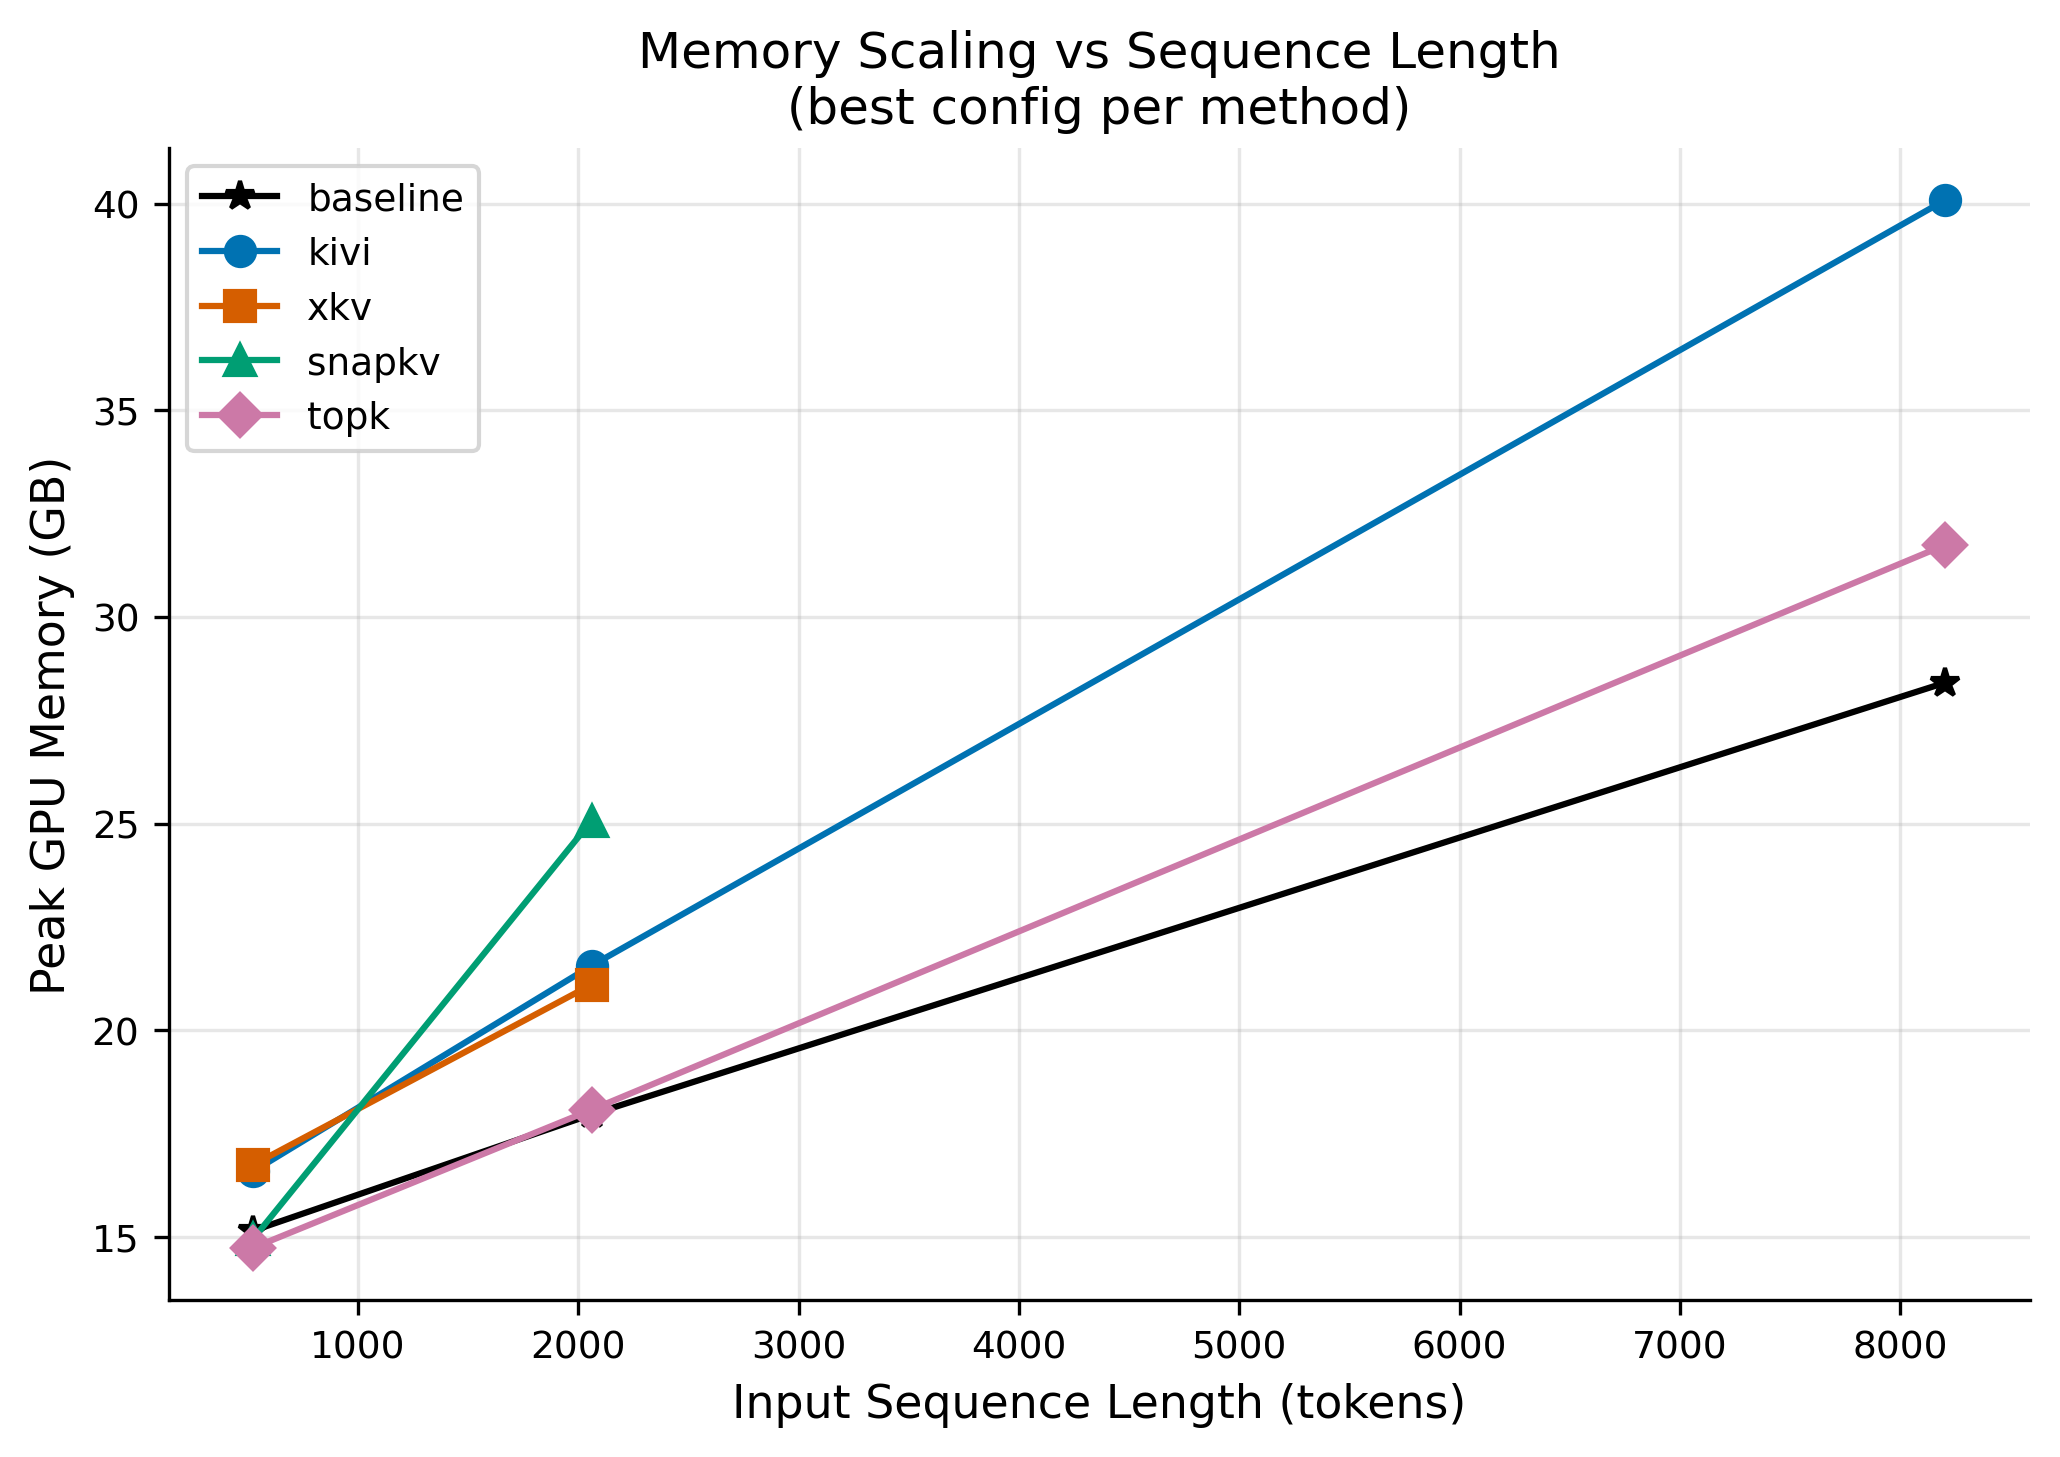
\includegraphics[width=\columnwidth]{../results/plots/memory_scaling.png}
    \caption{Left: KV cache size vs.\ sequence length---methods that compress (KIVI, SnapKV, xKV rank=64) show clear separation from baseline. Right: Peak GPU memory including model weights and temporaries---KIVI's dequantize-requantize overhead inflates peak memory despite smaller cache.}
    \label{fig:memory_scaling}
\end{figure}

\begin{figure}[t]
    \centering
    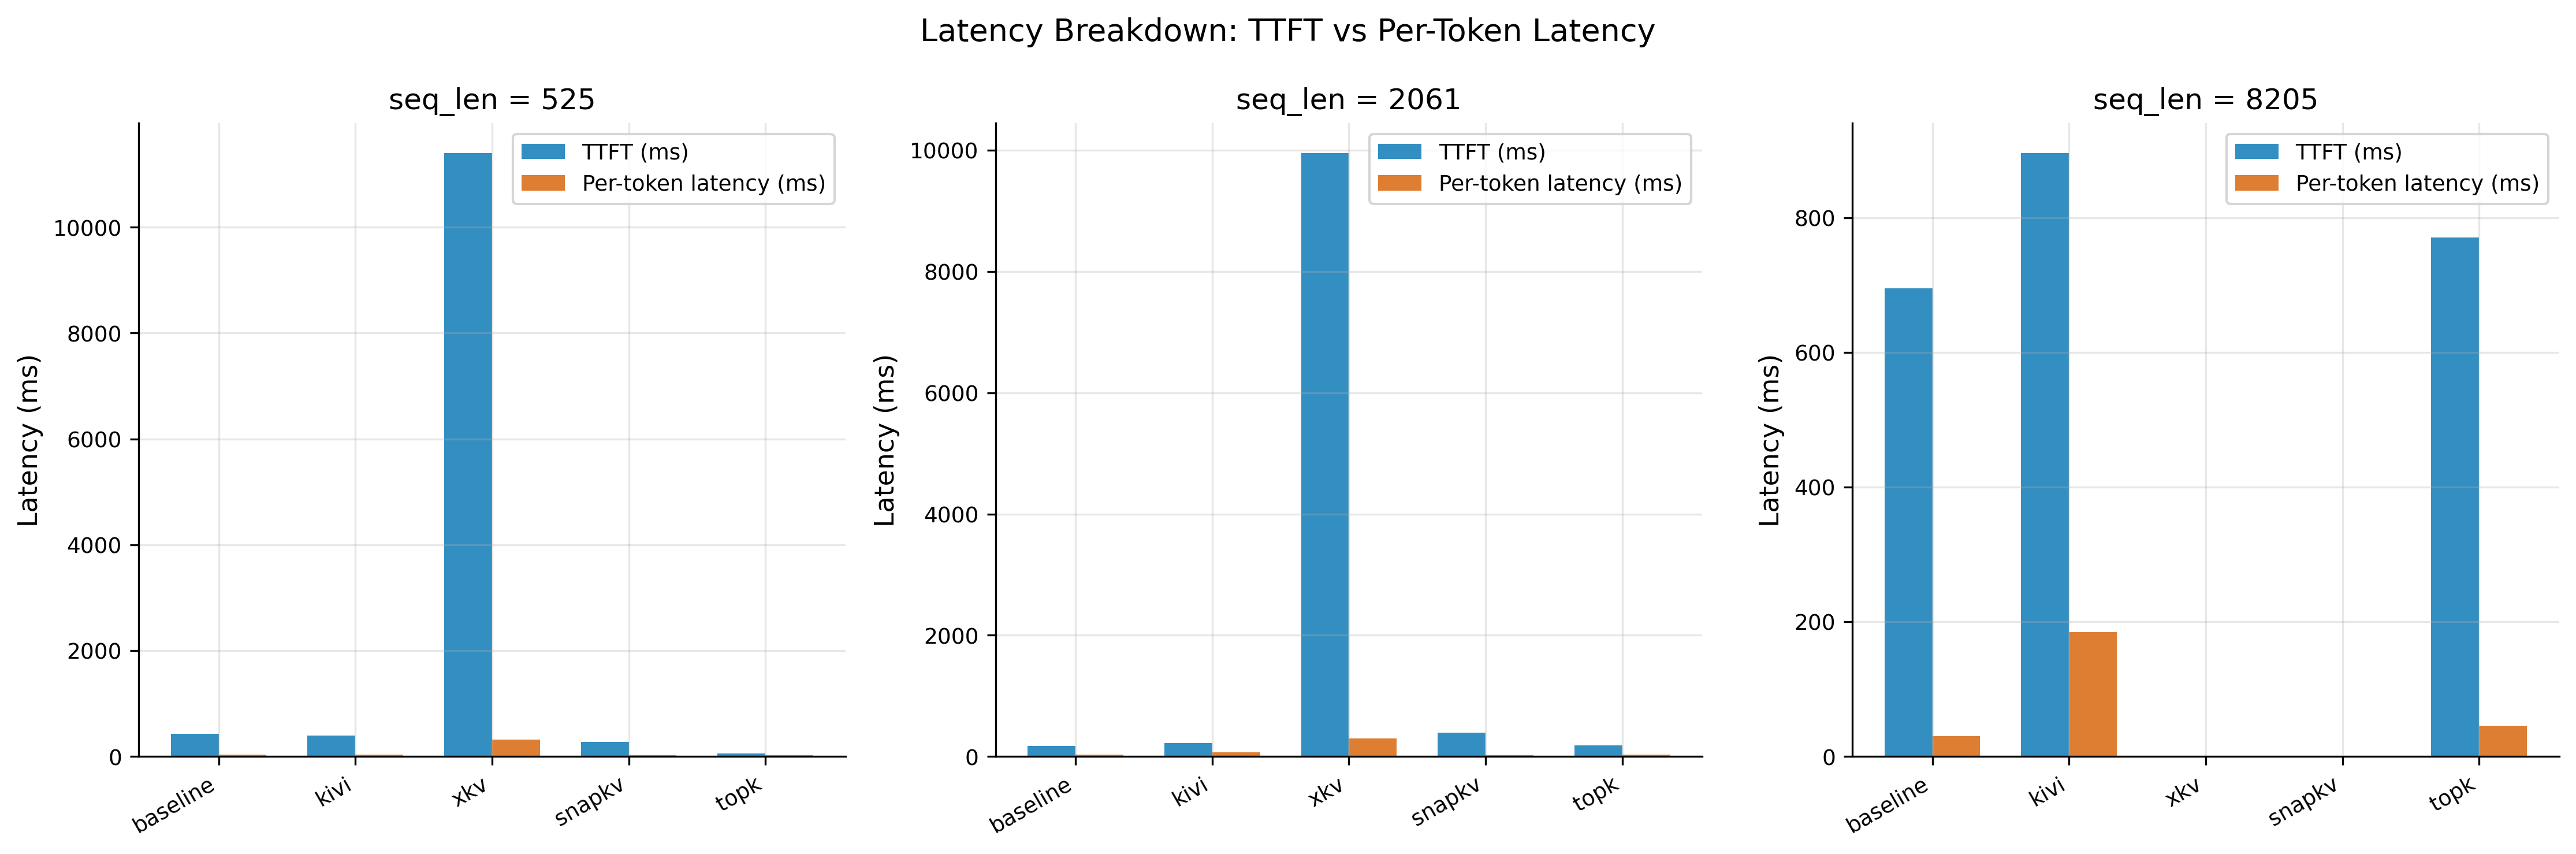
\includegraphics[width=\columnwidth]{../results/plots/latency_breakdown.png}
    \caption{Latency breakdown by sequence length: time-to-first-token (TTFT) vs.\ per-token decode latency. xKV exhibits extremely high TTFT due to initial SVD computation. KIVI shows elevated per-token latency from the requantization cycle.}
    \label{fig:latency}
\end{figure}

\subsection{Threats to Validity}

Several factors limit the generalizability of our findings:

\begin{itemize}
    \item \textbf{Single model}: Results are specific to LLaMA-2-7B. Methods may behave differently on architectures with grouped-query attention (e.g., LLaMA-3) or different head dimensions.
    \item \textbf{Batch size 1}: Production serving operates at higher batch sizes where KV cache memory pressure is amplified. The relative rankings may shift under batched workloads.
    \item \textbf{Greedy decoding}: We use deterministic argmax decoding. Sampling-based generation could interact differently with approximate KV caches since small probability perturbations may not affect argmax but could alter sampling outcomes.
    \item \textbf{Pure PyTorch}: The throughput results reflect unoptimized implementations. Methods with available optimized kernels (particularly KIVI) would show different absolute throughput numbers.
\end{itemize}

\section{Conclusion}

We presented a controlled benchmark of four KV cache optimization strategies evaluated under identical conditions on LLaMA-2-7B. Our key findings are:

\begin{enumerate}
    \item \textbf{Compression and quality are not always correlated}: KIVI 4-bit achieves 3.20$\times$ compression with no measurable quality loss, while SnapKV at 1.49$\times$ compression (budget=0.6) nearly doubles perplexity. The mechanism of compression---uniform quantization vs.\ selective eviction---determines quality impact more than the compression ratio itself.
    \item \textbf{Memory savings do not guarantee end-to-end efficiency}: KIVI compresses the KV cache by 5.27$\times$ but increases peak GPU memory by 27\% and reduces throughput by 56\% due to implementation overhead. Conversely, SnapKV reduces both cache size and computation, improving throughput by 52\%.
    \item \textbf{Quality-preserving methods exist but are limited}: TopK perfectly preserves quality while slightly improving throughput, but provides no memory savings. xKV rank=128 preserves quality but actually increases storage due to SVD component overhead exceeding savings.
    \item \textbf{The optimal choice is workload-dependent}: No single method dominates. Deployment decisions should be guided by the specific constraints (memory budget, latency SLA, quality threshold) of the target application.
\end{enumerate}

All code, results, and experiment configurations are available at \url{https://github.com/rishika1099/kv-cache-benchmark}. Interactive dashboards with per-run metrics are hosted at \url{https://wandb.ai/rm4318-columbia-university/kv-cache-benchmark}.

\bibliographystyle{IEEEtran}

\begin{thebibliography}{10}

\bibitem{kivi}
Z.~Liu, A.~Desai, F.~Liao, W.~Wang, V.~Xie, Z.~Xu, A.~Kyrillidis, and A.~Shrivastava, ``KIVI: A tuning-free asymmetric 2bit quantization for KV cache,'' in \textit{Proc. Int. Conf. Machine Learning (ICML)}, 2024.

\bibitem{xkv}
C.~Chang, W.~Lin, C.~Chen, and Y.~Tsvetkov, ``xKV: Cross-layer SVD for KV-cache compression,'' \textit{arXiv preprint arXiv:2503.18893}, 2025.

\bibitem{snapkv}
Y.~Li, Y.~Huang, B.~Yang, B.~Venkitesh, A.~Locatelli, H.~Ye, T.~Cai, P.~Lewis, and D.~Chen, ``SnapKV: LLM knows what you are looking for before generation,'' in \textit{Proc. Advances in Neural Information Processing Systems (NeurIPS)}, 2024.

\bibitem{topk}
Z.~Wu, P.~Zhong, Z.~Peng, and J.~Zhou, ``TokenSelect: Efficient long-context inference via dynamic token-level KV cache selection,'' in \textit{Proc. Conf. Empirical Methods in Natural Language Processing (EMNLP)}, 2025.

\bibitem{h2o}
Z.~Zhang, Y.~Sheng, T.~Zhou, T.~Chen, L.~Zheng, R.~Cai, Z.~Song, Y.~Tian, C.~R\'{e}, C.~Barrett, Z.~Wang, and B.~Chen, ``H2O: Heavy-hitter oracle for efficient generative inference of large language models,'' in \textit{Proc. Advances in Neural Information Processing Systems (NeurIPS)}, 2023.

\bibitem{pyramidkv}
Z.~Cai, Y.~Zhang, B.~Gao, Y.~Liu, T.~Liu, K.~Lu, W.~Xiong, Y.~Dong, B.~Chang, J.~Hu, and W.~Xiao, ``PyramidKV: Dynamic KV cache compression based on pyramidal information funneling,'' \textit{arXiv preprint arXiv:2406.02069}, 2024.

\bibitem{streamingllm}
G.~Xiao, Y.~Tian, B.~Chen, S.~Han, and M.~Lewis, ``Efficient streaming language models with attention sinks,'' in \textit{Proc. Int. Conf. Learning Representations (ICLR)}, 2024.

\bibitem{llama2}
H.~Touvron, L.~Martin, K.~Stone, P.~Albert, A.~Almahairi, Y.~Babaei, \textit{et al.}, ``Llama 2: Open foundation and fine-tuned chat models,'' \textit{arXiv preprint arXiv:2307.09288}, 2023.

\bibitem{vaswani}
A.~Vaswani, N.~Shazeer, N.~Parmar, J.~Uszkoreit, L.~Jones, A.~N.~Gomez, \L.~Kaiser, and I.~Polosukhin, ``Attention is all you need,'' in \textit{Proc. Advances in Neural Information Processing Systems (NeurIPS)}, 2017.

\bibitem{flashattention}
T.~Dao, D.~Fu, S.~Ermon, A.~Rudra, and C.~R\'{e}, ``FlashAttention: Fast and memory-efficient exact attention with IO-awareness,'' in \textit{Proc. Advances in Neural Information Processing Systems (NeurIPS)}, 2022.

\end{thebibliography}

\end{document}
